The found points will be used to compute the size-references which will be used to know the size of a ball and also to find the playing surface ROI.




\textbf{Using the points to find the cloth:}
The reason for finding the diamonds is to be able to find the exact ROI to search for the balls. This ROI is defined as 93.5mm from the diamond in a orthogonal line to the edge of the cushion, as seen in \ref{fig:diamonddistance}.

\begin{figure}[htpb]
\begin{center}
\leavevmode
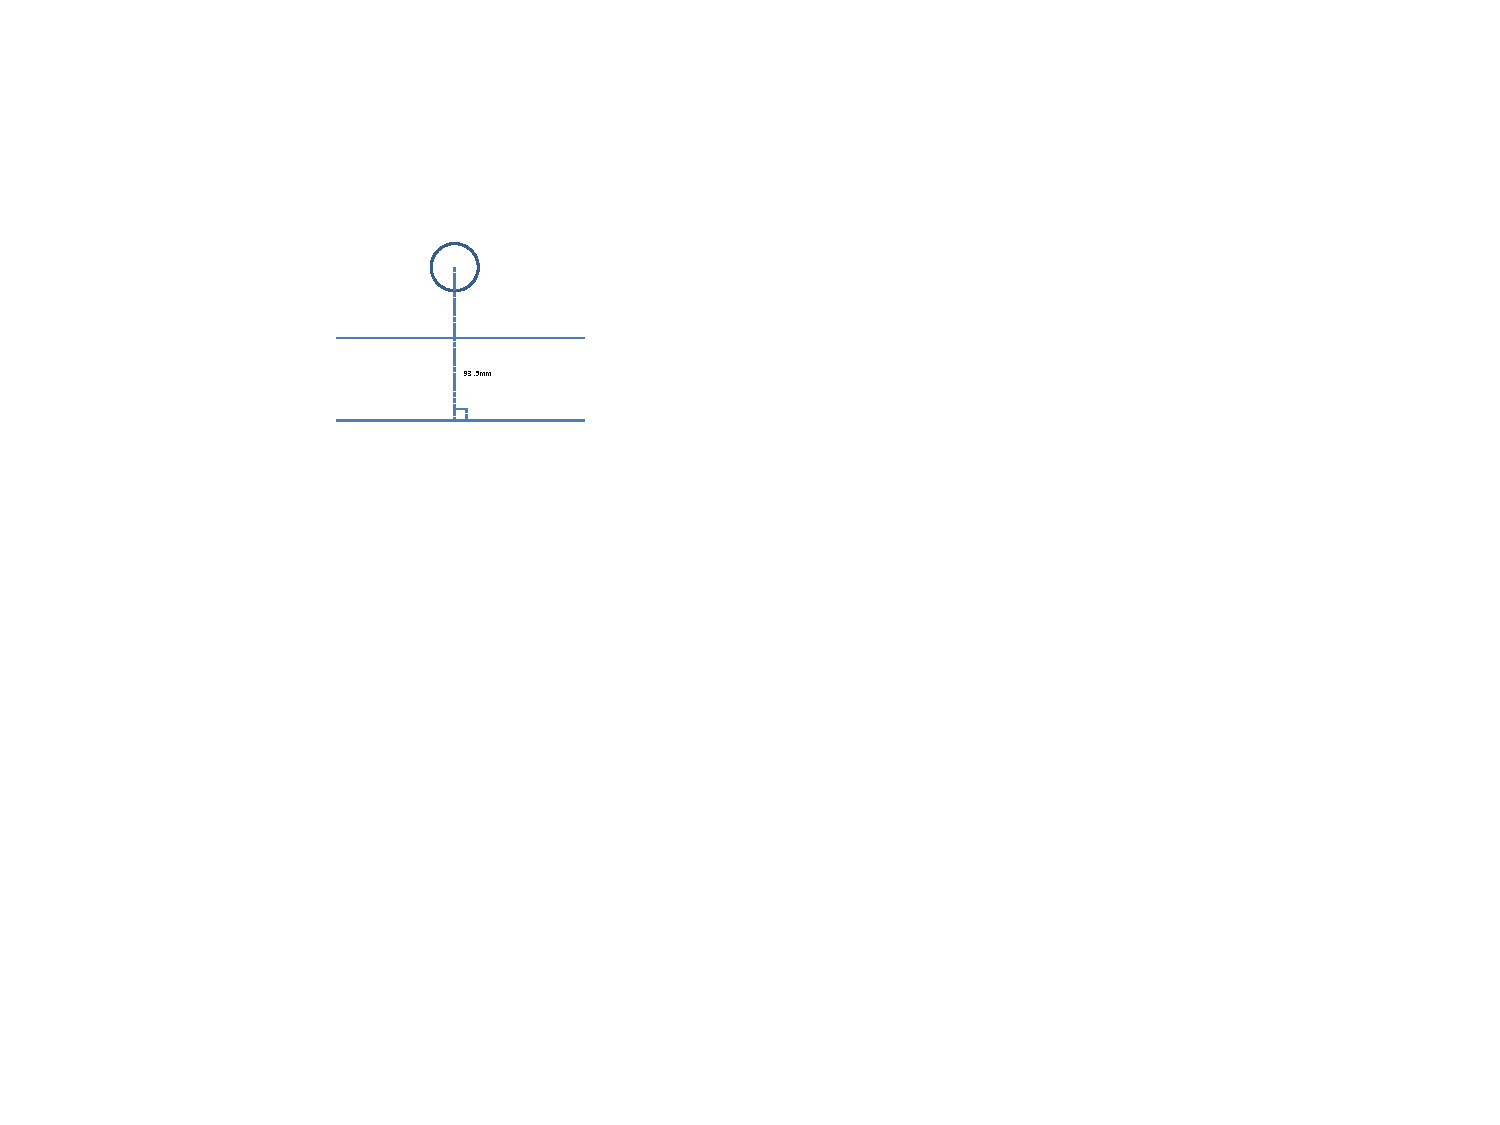
\includegraphics[width=0.5\textwidth]{images/diamonddistance.pdf}
\end{center}
\caption{Distance from diamond to nose of cushion.}
\label{fig:diamonddistance}
\end{figure}

